
\chapter{Graph Theory}
\label{chp:graph-theory}
\todo[inline,backgroundcolor=red!25]{Change Chapter to Background and include signed link prediction theory here as well}
In this chapter, we will provide the fundamentals of the graph theory concepts required to understand the rest of the thesis. In Section~\ref{sec:prelim} we cover the basic definitions and terminologies used to describe different types of graphs. Then we define a signed graph and discuss its unique properties in Section~\ref{sec:signed-graphs}. We outline the social theories of balance and status in signed networks in \Cref{sec:balance-theory,sec:status-theory}.\todo{Add line for link prediction} Lastly, we explain techniques of finding hierarchies in directed networks and the concept of agony in Section~\ref{sec:hierarchy}.

\section{Preliminaries}
\label{sec:prelim}
In this section, we define the various types of graphs and their basic properties. The notation and terminologies used closely follow those used in Diestel~\cite{diestel1997graph}. Graphs are structures that describe relationships between entities. These entities are called \textit{vertices} and entities related to one another are joined by edges. The terms graph, vertices and edges can be used interchangeably with \textit{network}, \textit{nodes} and \textit{links} respectively.

Graphs can be classified broadly into two types based on whether the edges posses a direction. We now go on to define them in detail.
\subsection{Undirected Graphs}
An undirected graph is pair $G=(V,E)$, where $V$ is the set of vertices and $E$ is the set $E \subseteq \{ (u,v) \mid u,v \in V\}$ of unordered pairs of vertices called edges. In this thesis we will deal only with \textit{simple graphs}, i.e. no self loops, $(u,v)\in V \times V, ~ u\neq v$ and there is at most one edge between vertices $u$ and $v$. 

The number of the vertices in a graph is called the \textit{order} of the graph and is denoted by $n= |G|$. In turn, the \textit{size} of a graph is the number of edges denoted by $m = \|G\|$ or $m=|E|$. A vertex $u$ is \textit{adjacent} to $v$ if they are the end points of an edge, $(u,v) \in E$. All the vertices adjacent to a vertex $v$ is called the \textit{neighbourhood} of $v$ and is denoted by $N(v)$. The \textit{degree} of a vertex $v$ is the number of nodes adjacent to that vertex and is denoted by $d(v) = |N(v)|$. 

The edges of an undirected graph can also have an associated value. This value can indicate the distance or similarity between a pair of vertices. These values are called \textit{weights} and the corresponding graph is called a \textit{weighted undirected graph}. Therefore, a weighted graph is defined as a triple $G=(V,E,w)$, where $w:E \rightarrow \mathbb{R}^{+}$ is a function that maps an edge $e$ to a positive real weight $w(e)$. Now an \textit{unweighted graph} is simply a weighted graph where the function $w$ is defined as: if $e \in E$ then $w(e)=1$ else $w(e)=0$. The degree of a vertex $v$ in a weighted graph is the sum of the weights to all the neighbours of $v$ and is defined as $d(v) = \sum_{u\in N(v)}w((u,v))$. An example of a weighted undirected graph is shown in Figure~\ref{fig:weighted-undirected}. 
\begin{figure}[!ht]
    \centering
    \tikzset{
    position/.style args={#1:#2 from #3}{
        at=(#3.#1), anchor=#1+180, shift=(#1:#2)
    }
}

\begin{tikzpicture}

    \begin{scope}[every node/.style={circle,thick,draw}]
        \node (v1) at (0,0) {$v_1$};
        \node[below=1cm of v1] (v2) {$v_2$};
        \node[position=45:2cm from v2] (v3) {$v_3$};
        \node[position=150:2cm from v1] (v4) {$v_4$};
        \node[left=3cm of v2] (v5) {$v_5$};
        \node[position=45:1cm from v5] (v6) {$v_6$};
    \end{scope}

    \begin{scope}[>={Stealth[red]},
        every edge/.style={thick,draw},
        every node/.style={fill=white,circle}]
        % \draw (v4) -- (v1) -- (v3) -- (v2) -- (v1);
        \path (v1) edge (v2) 
            (v2) edge (v3)
            (v1) edge node[above] {$1$} (v3)
            (v1) edge (v4)
            (v5) edge (v6)
            ;
    \end{scope}
  \end{tikzpicture}
  
    \caption{An example of a weighted undirected graph}
    \label{fig:weighted-undirected}
\end{figure}


\subsection{Directed Graphs}
The main distinction regarding a \textit{directed graph} (or \textit{digraph}) is that the edges are ordered pairs, i.e.$(u,v) \neq (v,u)$. Therefore, a directed graph has a similar definition: a pair $G=(V,E)$, where $V$ is the set of vertices and $E$ is the set of \textit{ordered} pairs of vertices. Now given an edge $e=(u,v)$ we can define a source function $\src:E\rightarrow V$ such that $\src(e)=u$ and a destination function $d:E\rightarrow V$ where $\dest(e)=v$. These functions classify the vertices in an edge $e$ as either the source or the destination. In this thesis, we deal only with \textit{simple directed graphs}, i.e. no self-loops, and there can be at most one edge from $u$ to $v$. 

As the edges now have an inherent direction, we can define the \textit{successors} and \textit{predecessors} of a node $v$. A vertex $u$ is called the \textit{successor} of a node $v$ if there exists a directed edge from $v$ to $u$, therefore the set of successors for a vertex $v$ can be defined as $S(v) = \{u \mid (v,u) \in E\}$. A \textit{predecessor} of a node $v$ is a vertex $u$ such that there exists a directed edge from $u$ to $v$, the set of predecessors for a vertex $v$ can de defined as $P(v) = \{u \mid (u,v) \in E\}$. Now, a vertex $u$ that is either a successor or a predecessor of a vertex $v$ can be called a neighbour of the vertex $v$. Therefore, we define the \textit{neighbourhood} of a vertex $v$ as the set of vertices in the union of successors and predecessor, i.e. $N(v) = S(u) \cup P(v)$. This definition is also compatible with undirected graphs because if $(u,v) \in E$ then $(v,u) \in E$. 

Directed graphs can also have values associated with each directed edge called a \textit{weight}. A \textit{weighted directed graph} can be defined as a triple $G=(V,E,w)$, where the weight function $w:E \rightarrow \mathbb{R}^{+}$ maps each edge $e$ to a weight $w(e)$. The indegree of a vertex $v$ is defined as the sum of the edge weights from the predecessors of $v$ and is denoted as $\indegree(v) = \sum_{u \in P(v)} w((u,v))$. Similarly, the outdegree of a vertex $v$ is defined as the sum of the edge weights to the successors of $v$ and is denoted by $\outdegree(v) = \sum_{u \in S(v)}w((v,u))$.
Figure~\ref{fig:weighted-directed} shows an example of a weighted directed graph.

\begin{figure}[!ht]
    \centering
    \tikzset{
    position/.style args={#1:#2 from #3}{
        at=(#3.#1), anchor=#1+180, shift=(#1:#2)
    }
}

\begin{tikzpicture}

    \begin{scope}[every node/.style={circle,thick,draw}]
        \node (v1) at (0,0) {$v_1$};
        \node[below=2cm of v1] (v2) {$v_2$};
        \node[right=2cm of v2] (v3) {$v_3$};
        \node[above=2cm of v3] (v4) {$v_4$};
        \node[below right=1cm and 2cm of v4] (v5) {$v_5$};
        \node[below left=1cm and 2cm of v1] (v6) {$v_6$};
    \end{scope}

    \begin{scope}[>={Stealth[black]},
        every edge/.style={thick,draw},
        every node/.style={fill=white,circle}]
        % \draw (v4) -- (v1) -- (v3) -- (v2) -- (v1);
        \path[->] 
        (v1) edge[bend right=20] node[left] {$2$} (v2)
        (v2) edge[bend right=30] node[below right=1mm] {$4$} (v4)  
        (v1) edge[bend left=35] node[above=0.8mm] {$1$} (v4)
        (v4) edge[bend left=35] node[below=0.8mm] {$1.5$} (v1)
        (v5) edge[bend left=30] node[below right=1mm] {$3.5$} (v3)
        (v2) edge[bend left=30] node[below left=0.8mm and 0.8mm] {$2.5$} (v6)
        ;
    \end{scope}
  \end{tikzpicture}
  
    \caption{An example of a weighted directed graph}
    \label{fig:weighted-directed}
\end{figure}

\section{Signed Graphs}
\label{sec:signed-graphs}
The simple weighted graphs we have defined so far only have non-negative edge weights that can represent similarity or closeness. In the 1950s, social psychologists found it desirable to express liking, disliking or indifference in social interactions. This was formalized by Harary \cite{harary1953on} using graphs with weights $(-1,0,1)$. These graphs are therefore called \textit{signed graphs}, where a negative edge weight can denote dissimilarity between a pair of vertices. In this thesis we will use notations and terms similar to Gallier \cite{gallier2016spectral}, Kunegis et al. \cite{kunegis2010spectral}, Hou \cite{hou2005bounds} and Zaslavsky \cite{zaslavsky1982signed}.

A signed graph is a triple $G=(V,E,w)$, where $V$ is the set of vertices, $E$ is the set of pairs of vertices and the weight function $w:E \rightarrow \mathbb{R}$. The weight function now takes an edge $e$ and maps it to a signed weight $w(e)$. We can partition the edges into positive and negative edges, $E = E^{+}\cup E^{-}$, where $E^{+} = \{e \mid w(e)>0\}$ and $E^{-}=\{e \mid w(e)<0\}$. Similar to Zaslavsky \cite{zaslavsky1982signed}, we consider undirected signed graphs and directed signed graphs as distinct and separate entities. We can see some examples of signed graphs in Figure~\ref{fig:signed-graphs}.
\begin{figure}[!ht]
    \centering
    \begin{subfigure}{0.5\textwidth}
        \centering
        \tikzset{
    position/.style args={#1:#2 from #3}{
        at=(#3.#1), anchor=#1+180, shift=(#1:#2)
    }
}

\begin{tikzpicture}

    \begin{scope}[every node/.style={circle,thick,draw}]
        \node (v1) at (0,0) {$v_1$};
        \node[below=1cm of v1] (v2) {$v_2$};
        \node[position=45:2cm from v2] (v3) {$v_3$};
        \node[position=150:2cm from v1] (v4) {$v_4$};
        \node[left=3cm of v2] (v5) {$v_5$};
        \node[position=45:1.3cm from v5] (v6) {$v_6$};
    \end{scope}

    \begin{scope}[>={Stealth[red]},
        every edge/.style={thick,draw},
        every node/.style={fill=white,rectangle}]
        % \draw (v4) -- (v1) -- (v3) -- (v2) -- (v1);
        \path (v1) edge node[left] {$2$} (v2) 
            (v2) edge node[below right=0.05cm and 0.05cm] {$-1.5$} (v3)
            (v1) edge node[above=0.05cm] {$-1$} (v3)
            (v1) edge node[above right] {$4$} (v4)
            (v5) edge node[above left] {$-3$} (v6)
            ;
    \end{scope}
  \end{tikzpicture}
  
        \caption{A undirected signed graph}
        \label{fig:signed-undirected}
    \end{subfigure}

    \begin{subfigure}{0.5\textwidth}
        \centering
        \tikzset{
    position/.style args={#1:#2 from #3}{
        at=(#3.#1), anchor=#1+180, shift=(#1:#2)
    }
}

\begin{tikzpicture}

    \begin{scope}[every node/.style={circle,thick,draw}]
        \node (v1) at (0,0) {$v_1$};
        \node[below=2cm of v1] (v2) {$v_2$};
        \node[right=2cm of v2] (v3) {$v_3$};
        \node[above=2cm of v3] (v4) {$v_4$};
        \node[below right=1cm and 2cm of v4] (v5) {$v_5$};
        \node[below left=1cm and 2cm of v1] (v6) {$v_6$};
    \end{scope}

    \begin{scope}[>={Stealth[black]},
        every edge/.style={thick,draw},
        every node/.style={fill=white,rectangle}]
        % \draw (v4) -- (v1) -- (v3) -- (v2) -- (v1);
        \path[->] 
        (v1) edge[bend right=20] node[left=0.05cm] {$-2$} (v2)
        (v2) edge[bend right=30] node[below right=1mm] {$4$} (v4)  
        (v1) edge[bend left=35] node[above=0.8mm] {$-1$} (v4)
        (v4) edge[bend left=35] node[below=0.8mm] {$1.5$} (v1)
        (v5) edge[bend left=30] node[below right=1mm] {$3.5$} (v3)
        (v2) edge[bend left=30] node[below left=0.8mm and 0.8mm] {$2.5$} (v6)
        ;
    \end{scope}
  \end{tikzpicture}
  
        \caption{A directed signed graph}
        \label{fig:signed-directed graph}
    \end{subfigure}
    \caption{Examples of Signed Graphs}
    \label{fig:signed-graphs}
\end{figure}

We can now proceed to define a few more terms. The degree of a vertex $v$ is now the sum of the absolute edge weight of its neighbours, called the \textit{signed degree} and is defined as 
\[
    \overline{d}(v) = \sum_{u \in N(v)}|w((u,v))|
\] 
This can also be extended to \textit{signed indegree} and \textit{signed outdegree} denoted by $\overline{\indegree}(v)$ and $\overline{\outdegree}(v)$ and defined as
\[
    \overline{\indegree}(v)=\sum_{u \in P(v)}|w((u,v))|
\] 
\[
    \overline{\outdegree}(v)=\sum_{u \in S(v)}|w((v,u))|
\] 

We can create a $n \times n$ square weight matrix $W$, where each entry $w_{ij}$ is defined as 

\[ w_{ij} = 
\begin{cases}
    w((v_i,v_j)) & \text{if } (v_i,v_j) \in E \\
    0 & \text{if } (v_i,v_j) \notin E      
\end{cases}
\] 
The signed degree matrix $\overline{D}$ is a diagonal matrix consisting of the signed verted degrees, $\overline{D} = \text{diag}(\overline{d}(v_{1}),\dots,d(v_n))$. We can now define the \textit{signed Laplacian}, $\overline{L}$ as 
\[ \overline{L} = \overline{D} - W\]
The signed Laplacian along with results from spectral analysis of signed graphs \cite{hou2005bounds,kunegis2010spectral}, will be useful for balance theory of signed graphs. 

\subsection{Balance Theory}
\label{sec:balance-theory}


In the 1940s, Heider \cite{heider1946attitudes} proposed  that when there are either \textit{positive relations} (friendship, love, support) and \textit{negative relations} (enmity, hate, oppose) in a group, the  group tends towards \textit{balance}. Balance is the concept that all members aim to maintain consistency in the relations they share with other members of the group. In a group of three members this can be seen as having three positive relations or one positive and two negative relations. In Figure~\ref{fig:undirected-triads} the triads $B_1$ and $B_2$ are \textit{balanced} and mirror aphorisms such as "the friend of my friend is also a friend" and "the enemy of my enemy is a friend" respectively. Therefore, triads $B_3$ and $B_4$ can be called \textit{unbalanced} or \textit{imbalanced} that denotes the cognitive dissonance between the members of the triad. The dissonance can be understood by the counterintuitive nature of the phrase "the friend of my friend is my enemy" described by triad $B_3$.

Harary and Cartwright \cite{cartwright1956structural} generalized this notion of balance by using signed graphs. As these relations are typically symmetric, balance is usually defined for undirected signed graphs. This can been seen in Figure~\ref{fig:undirected-triads} where solid edges are positive and dashed edges are negative. Davies \cite{davis1963weakBalance} also offers an alternate definition of \textit{weak balance} where triads of type $B_2$ are considered to have lesser predictive utility as relationships of these type are less common in real-life social networks.

\begin{figure}[!ht]     
    \centering
    \tikzset{
    position/.style args={#1:#2 from #3}{
        at=(#3.#1), anchor=#1+180, shift=(#1:#2)
    }
}

\begin{tikzpicture}

    \begin{scope}[every node/.style={circle,thick,draw}]
        \node (v1) at (0,0) {};
        \node[position=-120:1cm from v1] (v2) {};
        \node[position=-60:1cm from v1] (v3) {};
        
        \node[right=2cm of v1] (v4) {};
        \node[position=-120:1cm from v4] (v5) {};
        \node[position=-60:1cm from v4] (v6) {};
        
        \node[right=2cm of v4] (v7) {};
        \node[position=-120:1cm from v7] (v8) {};
        \node[position=-60:1cm from v7] (v9) {};
        
        \node[right=2cm of v7] (v10) {};
        \node[position=-120:1cm from v10] (v11) {};
        \node[position=-60:1cm from v10] (v12) {};
        

    \end{scope}

    \begin{scope}[>={Stealth[red]},
        positive/.style={thick,draw},
        negative/.style={thick,dashed,draw},
        every node/.style={fill=white,circle}]
        % \draw (v4) -- (v1) -- (v3) -- (v2) -- (v1);
        \path 
        (v1) edge[positive] node[above left=0.1mm and 0.1mm] {$+$} (v2)
        (v1) edge[positive] node[above right=0.1mm and 0.1mm] {$+$} (v3) 
        (v3) edge[positive] node[below] {$+$} node[below=1cm] {$T_1$}  (v2)      
        ;
        \path 
        (v4) edge[negative] node[above left=0.1mm and 0.1mm] {$-$} (v5)
        (v4) edge[negative] node[above right=0.1mm and 0.1mm] {$-$} (v6) 
        (v6) edge[positive] node[below] {$+$} node[below=1cm] {$T_2$}  (v5)      
        ;
        \path 
        (v7) edge[positive] node[above left=0.1mm and 0.1mm] {$+$} (v8)
        (v7) edge[positive] node[above right=0.1mm and 0.1mm] {$+$} (v9) 
        (v9) edge[negative] node[below] {$-$} node[below=1cm] {$T_3$}  (v8)      
        ;
        \path 
        (v10) edge[negative] node[above left=0.1mm and 0.1mm] {$-$} (v11)
        (v10) edge[negative] node[above right=0.1mm and 0.1mm] {$-$} (v12) 
        (v12) edge[negative] node[below] {$-$} node[below=1cm] {$T_4$}  (v11)      
        ;
    \end{scope}
  \end{tikzpicture}
    
    \caption{Triads in undirected signed graphs. $B_1$ and $B_2$ are \textit{balanced} triads as they have even number of negative edges. $B_3$ and $B_4$ are \textit{unbalanced} as they have odd number of negative edges.}
    \label{fig:undirected-triads}
\end{figure}

The concept of balance can be generalized for an undirected signed graph $G=(V,E,w)$. The sign of a cycle $C$ in the signed graph $G$ is defined as the product of the edge weights $sgn(C)=\prod_{e\in C}w(e)$. A signed network $G$ is then said to be balanced if and only if all the sign of all cycles in network are positive. Therefore, every cycle in $G$ must have an even number of negative edges. This leads to result from Harary \cite{harary1953on} that states that if a graph $G$ is balanced, then there is a partition of the vertices $V = V_1 \cup V_2$ such that edges within the vertices of each set is positive and edges between the sets are negative. This means that we can have a bipartite graph when we delete the positive edges and negative edges span between the two sets of vertices. An example of a balanced signed graph is shown in Figure~\ref{fig:balanced-graph}. Here the partition of the vertex set is $V_1 = \{v_1,v_3,v_4,v_7,v_8\}$ and $V_2 = \{v_2,v_5,v_6,v_9\}$.

\begin{figure}[!ht]
    \centering
    \tikzset{
    position/.style args={#1:#2 from #3}{
        at=(#3.#1), anchor=#1+180, shift=(#1:#2)
    }
}

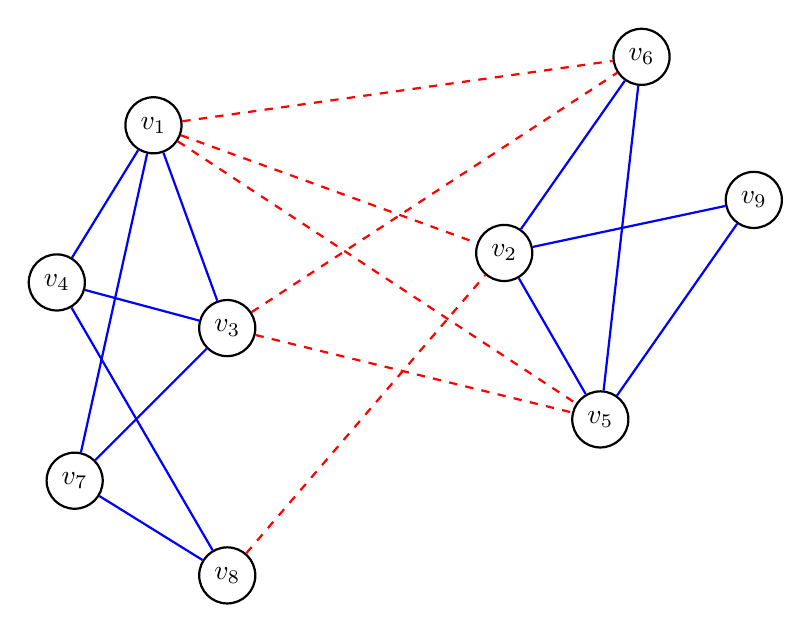
\begin{tikzpicture}

    \begin{scope}[every node/.style={circle,thick,draw}]
        \node (v1) at (0,0) {$v_1$};
        \node[position=-20:4cm from v1] (v2) {$v_2$};
        \node[position=-60:1.7cm from v2] (v5) {$v_5$};
        \node[position=55:2.3cm from v2] (v6) {$v_6$};
        \node[position=12:2.5cm from v2] (v9) {$v_9$};
        \node[position=-70:2cm from v1] (v3) {$v_3$};
        \node[position=-195:1.5cm from v3] (v4) {$v_4$};
        \node[position=225:2cm from v3] (v7) {$v_7$};
        \node[position=-90:2.4cm from v3] (v8) {$v_8$};
    \end{scope}

    % positive edges
    \begin{scope}[every edge/.style={thick,draw,blue},
        every node/.style={fill=white,circle}]
        % \draw (v4) -- (v1) -- (v3) -- (v2) -- (v1);
        \path 
        (v2) edge (v5) 
        (v5) edge (v9)
        (v2) edge (v6)
        (v6) edge (v5)
        (v2) edge (v9)      
        (v1) edge (v3)
        (v1) edge (v4)
        (v4) edge (v3)
        (v3) edge (v7)
        (v7) edge (v1)
        (v4) edge (v8)
        (v8) edge (v7)
        ;
    \end{scope}
    % negative edges
    \begin{scope}[every edge/.style={thick,draw,red,dashed},
        every node/.style={fill=white,circle}]
        % \draw (v4) -- (v1) -- (v3) -- (v2) -- (v1);
        \path 
        (v1) edge (v2)
        (v1) edge (v6)
        (v3) edge (v6)
        (v3) edge (v5)
        (v8) edge (v2)
        (v1) edge (v5)
        ;
    \end{scope}
  \end{tikzpicture}
  
    \caption{ A balanced signed graph. Solid blue edges are positive and dashed red edges are negative. Every cycle in this graph contains an even number of negative edges.}
    \label{fig:balanced-graph}
\end{figure}

The signed Laplacian matrix $\overline{L}$ of a signed graph $G$ is always positive-semidefinite and $\overline{L}$ is positive-definite iff $G$ is \textit{unbalanced} \cite{kunegis2010spectral,hou2005bounds,zaslavsky1982signed}. If the smallest eigenvalue of a graph $G$ is denoted by $\lambda_{1}(G)$, then $G$ is balanced iff $\lambda_{1}(G)=0$. Hou \cite{hou2005bounds} provides bounds on the value of $\lambda_{1}(G)$ and Li et al. \cite{li2016note} show that $\lambda_{1}(G)$ can be used as a measure of how far the signed graph $G$ is from being balanced.

\subsection{Status Theory}
\label{sec:status-theory}
Guha et al. \cite{guha2004propagation} mention implicitly that a signed edge from $u$ to $v$ can be interpreted in a asymmetric manner different from "friend" or "enemy". Leskovec et al. \cite{leskovec2010signed,leskovec2010predicting} introduce the concept of \textit{status} to contextualize directed singed edges. A positive edge $u \xrightarrow{+} v$ indicates that $v$ has a higher status than $u$ and a negative edge $u \xrightarrow{-} v$ means that $v$ has a lower status than $u$. This concept of relative status can be propagated transitively along multiple steps which might lead to contradictions with balance theory \cite{leskovec2010signed}.

Given three vertices $v_1,v_2$ and $v_3$, the presence of an edge $v_1 \xrightarrow{+} v_2$ indicates that $v_1$ thinks $v_2$ has higher status, the edge $v_2 \xrightarrow{+} v_3$ indicates that $v_2$ thinks $v_3$ has higher status. Now we wish to to close this triad with an edge from $v_3$ to $v_1$. Status theory would say that through transitivity $v_1$ has lower status than $v_3$, therefore the prediction is $v_3 \xrightarrow{-} v_1$. Whereas, in balance theory we would predict a positive edge $v_3 \xrightarrow{+} v_1$ to make the cycle have even number of negative edges. This example can be seen in triads $S_1$ and $S_2$ shown in Figure~\ref{fig:status-triads}.

There are also cases when status theory is ambivalent to the edge that closes a triad. Consider the example when we have the edges $v_1 \xrightarrow{+} v_2$ and $v_2 \xrightarrow{-} v_3$. If we were to indicate the status of a vertex $v$ using the function $s(v)$, then the edges describe the following : $s(v_2)>s(v_1) $ and $s(v_2)>s(v_3)$. Therefore, we have no knowledge of the relative difference in status between the vertices $v_1$ and $v_3$. Hence, both edges $v_3 \xrightarrow{+} v_1$ ($s(v_3) > s(v_1)$) and $v_3 \xrightarrow{-} v_1$ ($s(v_1) > s(v_3)$) are equally valid for status theory. Balance theory on the other hand can only predict $v_3 \xrightarrow{-} v_1$ to keep the triad balanced. This case is shown in Figure~\ref{fig:status-triads} as triads $S_3$ and $S_4$.

\begin{figure}[!ht] 
    \centering
    \tikzset{
    position/.style args={#1:#2 from #3}{
        at=(#3.#1), anchor=#1+180, shift=(#1:#2)
    }
}

\begin{tikzpicture}

    \begin{scope}[every node/.style={circle,thick,draw}]
        \node (v2) at (0,0) {$v_2$};
        \node[position=-120:1cm from v2] (v1) {$v_1$};
        \node[position=-60:1cm from v2] (v3) {$v_3$};
        
        \node[right=2.5cm of v2] (v5) {$v_2$};
        \node[position=-120:1cm from v5] (v4) {$v_1$};
        \node[position=-60:1cm from v5] (v6) {$v_3$};
        
        \node[right=2.5cm of v5] (v8) {$v_2$};
        \node[position=-120:1cm from v8] (v7) {$v_1$};
        \node[position=-60:1cm from v8] (v9) {$v_3$};
        
        \node[right=2.5cm of v8] (v11) {$v_2$};
        \node[position=-120:1cm from v11] (v10) {$v_1$};
        \node[position=-60:1cm from v11] (v12) {$v_3$};
        

    \end{scope}

    \begin{scope}[>={Stealth[black]},
        positive/.style={thick,draw,->},
        negative/.style={thick,dashed,draw,->},
        every node/.style={fill=white,circle}]
        % \draw (v4) -- (v1) -- (v3) -- (v2) -- (v1);
        \path 
        (v1) edge[positive] node[above left=0.1mm and 0.1mm] {$+$} (v2)
        (v2) edge[positive] node[above right=0.1mm and 0.1mm] {$+$} (v3) 
        (v3) edge[positive] node[below] {$+$} node[below=1cm] {$S_1$}  (v1)      
        ;
        \path 
        (v4) edge[positive] node[above left=0.1mm and 0.1mm] {$+$} (v5)
        (v5) edge[positive] node[above right=0.1mm and 0.1mm] {$+$} (v6) 
        (v6) edge[negative] node[below] {$-$} node[below=1cm] {$S_2$}  (v4)      
        ;
        \path 
        (v7) edge[positive] node[above left=0.1mm and 0.1mm] {$+$} (v8)
        (v8) edge[negative] node[above right=0.1mm and 0.1mm] {$-$} (v9) 
        (v9) edge[negative] node[below] {$-$} node[below=1cm] {$S_3$}  (v7)      
        ;
        \path 
        (v10) edge[positive] node[above left=0.1mm and 0.1mm] {$+$} (v11)
        (v11) edge[negative] node[above right=0.1mm and 0.1mm] {$-$} (v12) 
        (v12) edge[positive] node[below] {$+$} node[below=1cm] {$S_4$}  (v10)      
        ;
    \end{scope}
  \end{tikzpicture}
  
    \caption{Triads in directed signed graphs. Triads $S_2,S_3$ and $S_4$ are compliant with status theory. Only triads $S_1$ and $S_3$ are compliant with balance theory.}
    \label{fig:status-triads}
\end{figure}

Each positive link inwards ($\indegree^{+}(v)$) and negative link outwards ($\outdegree^{-}(v)$) increases status. Each positive link outwards ($\outdegree^{+}(v)$) and negative link inwards ($\indegree^{-}(v)$) decreases status. Therefore, $\sigma(v) = \indegree^{+}(v) + \outdegree^{-}(v) - \outdegree^{+}(v)- \indegree^{-}(v)$ is a heuristic for the status of a node \cite{leskovec2010predicting}. An interesting fact is that the edge $u \xrightarrow{-} v$ can be converted into positive edge in the opposite direction $u \xleftarrow{+} v$. This fact reduces the number of unique triads that can be formed using status theory and will be used in edge prediction tasks that will be discussed in coming chapters.

\section{Hierarchy in directed networks}
\label{sec:hierarchy}
Hierarchies exist in all social structures, from the explicit levels found in nature such as the food chain or organizational structures in businesses to more implicit stratification that occurs on social media or online networks. A common method to represent such hierarchies is through a tree, for example, the chain of command in the military or within governments. Trees have well defined levels and a single person at the top. If we generalize this structural concept then we get a \textit{Directed Acyclic Graph} (DAG) which represents a partial ordering set. DAGs have perfect hierarchy while structures such as cycles tend to have no hierarchy. Other directed graphs occur somewhere between these two extremes.

Gupte et al. \cite{gupte2011finding} provide a method to discern the levels of stratification present in a given directed network when no prior information of the hierarchy exists. They define a measure of the hierarchy of a given directed network $G$ as $h(G)$ along with a polynomial algorithm to find the largest hierarchy in that network. They define a concept of \textit{social agony} which posits that agony is present when a person having a higher rank in network interacts with a person who has a lower rank. Therefore, if we define the rank of a node in graph $G$ as the function $r:V \rightarrow \mathbb{N}$, then a directed edge $u \rightarrow v$ causes agony when $r(u)\geq r(v)$. The agony for the edge can be quantified as $\max(r(u)-r(v)+1,0)$. The agony of the graph $G$ wrt to rank function $r$ is defined as 
\[A(G,r) =  \sum_{(u,v)\in E} \max(r(u)-r(v)+1,0)\]
As nodes in a graph tend to minimize the overall agony, the agony of a network $G$ is the smallest possible agony over all possible ranking for $r$, $A(G) = \min_{r\in \text{Rankings}}A(G,r)$. The hierarchy of a given network $G$, denoted by $h(G)$ can now be expressed in terms of the agony of the network, $h(G)=1-\frac{1}{m}A(G)$, where $m$ is the number of edges. We can see examples of hierarchy in unweighted directed graph in Figure~\ref{fig:hierarchy}.

 
\begin{figure}[!ht]
    \centering
    \begin{subfigure}[t]{0.5\textwidth}
        \centering
        \tikzset{
    position/.style args={#1:#2 from #3}{
        at=(#3.#1), anchor=#1+180, shift=(#1:#2)
    }
}

\begin{tikzpicture}

    \begin{scope}[every node/.style={circle,thick,draw}]
        \node (v1) at (0,0) {$1$};
        \node[right=1.5cm of v1] (v2) {$1$};
        \node[right=1.5cm of v2] (v3) {$1$};
        \node[above=1cm of v2] (v5) {$2$};
        \node[left=3cm of v5] (v4) {$2$};
        \node[right=2.5cm of v5] (v6) {$2$};
        \node[above right=1cm and 1.5cm of v4] (v7) {$3$};
        \node[above=2cm of v4] (v8) {$4$};
        \node[right=5cm of v8] (v9) {$4$};
    \end{scope}

    \begin{scope}[>={Stealth[black]},
        every edge/.style={thick,draw,->},
        every node/.style={fill=white,circle}]
        % \draw (v4) -- (v1) -- (v3) -- (v2) -- (v1);
        \path 
        (v1) edge (v4)
        (v1) edge (v7)
        (v1) edge (v5)
        (v2) edge (v5)
        (v3) edge (v5)
        (v3) edge (v6)
        (v3) edge (v9)
        (v4) edge (v7)
        (v4) edge (v8)
        (v5) edge (v7)
        (v6) edge (v9)
        (v7) edge (v8)
        (v7) edge (v9)

        ;
    \end{scope}
  \end{tikzpicture}
  
        \caption{DAG has perfect hierarchy, $h(G)=1$ and agony of each edge is 0}
        \label{fig:dag}
    \end{subfigure}

    \begin{subfigure}[t]{0.49\textwidth}
        \centering
        \tikzset{
    position/.style args={#1:#2 from #3}{
        at=(#3.#1), anchor=#1+180, shift=(#1:#2)
    }
}

\begin{tikzpicture}

    \begin{scope}[every node/.style={circle,thick,draw}]
        \node (v1) at (0,0) {$1$};
        \node[right=1.5cm of v1] (v2) {$1$};
        \node[above=1.5cm of v2] (v3) {$1$};
        \node[left=1.5cm of v3] (v4) {$1$};

    \end{scope}

    \begin{scope}[>={Stealth[black]},
        every edge/.style={thick,draw,->},
        every node/.style={fill=white,circle}]
        % \draw (v4) -- (v1) -- (v3) -- (v2) -- (v1);
        \path 
        (v1) edge (v2)
        (v2) edge (v3)
        (v3) edge (v4)
        (v4) edge (v1)

        ;
    \end{scope}
  \end{tikzpicture}
  
        \caption{Cycle has no hierarchy, $h(G)=0$ and each edge has agony of 1}
        \label{fig:cycle}
    \end{subfigure}
    \begin{subfigure}[t]{0.49\textwidth}
        \centering
        \tikzset{
    position/.style args={#1:#2 from #3}{
        at=(#3.#1), anchor=#1+180, shift=(#1:#2)
    }
}

\begin{tikzpicture}

    \begin{scope}[every node/.style={circle,thick,draw}]
        \node (v1) at (0,0) {$1$};
        \node[right=2cm of v1] (v2) {$1$};
        \node[above right=1.5cm of v1] (v3) {$2$};
        \node[above left = 1.5cm of v3] (v4) {$3$};
        \node[above right=1.5cm of v3] (v5) {$3$};
    \end{scope}

    \begin{scope}[>={Stealth[black]},
        every edge/.style={thick,draw,->},
        back/.style ={very thick,dashed,red,->},
        every node/.style={fill=white,circle}]
        % \draw (v4) -- (v1) -- (v3) -- (v2) -- (v1);
        \path 
        (v1) edge (v3)
        (v1) edge (v4)
        (v2) edge (v3)
        (v3) edge (v5)
        (v5) edge[back,bend left] (v2)
        ;
    \end{scope}
  \end{tikzpicture}
  
        \caption{Graph with some hierarchy $h(G)=\frac{2}{5}$. Red dashed edge has agony of 3 and solid black edges have 0 agony.  }
        \label{fig:some-hierarchy}
    \end{subfigure}
    \caption{Examples of hierarchy in unweighted directed graphs. Numbers inside nodes indicate the rank of vertex.}
    \label{fig:hierarchy} 
\end{figure}

Therefore, finding a ranking of the nodes that minimizes the agony of the network gives us the optimal hierarchy present in that network. Gupte et al. \cite{gupte2011finding} and Tatti \cite{tatti2014faster} present a polynomial algorithm that can solve the dual of the agony minimization problem to obtain the optimal ranking $r$ for unweighted graphs. Tatti \cite{tatti2017tiers} provides an alternate approach using a capacitated circulation solver that can handle weighted digraphs as well as additional cardinality constraints. These algorithms allows us to find the levels of hierarchy present in any given directed social network and analyse the interaction between members belonging to different strata in that community.

We will explain in future chapters how hierarchies in social network is intrinsically linked to the theory of status in directed signed networks. We show one can use the concept of agony of a directed signed graph $G$ to quantify the violation to status theory and use it as a metric to predict an unknown signed edge.

\section{Link and Sign Prediction}
\label{sec:link-prediction}
The \textit{link prediction problem} is defined by Liben-Nowell and Kleinberg \cite{liben-nowell2007the} as inferring possible future edges between vertices in a social network. The datasets used was split into training edges and testing edges which had a common core set of vertices. They showed that topological features such as number of common neighbours and Katz's centrality index can be used in a unsupervised setting to accurately predict edges.

Leskovec et al. \cite{leskovec2010predicting} extended the link prediction problem to signed networks. They also introduced the problem of \textit{edge sign prediction}: predict the sign of a given edge $(u,v)$ using the existing signed network $G$. A supervised model for the task is proposed that uses network features such as indegree and outdegree of a node along with \textit{triad} features. The edge nodes $u$ and $v$ and a common neighbour $w$ form a triad. The directed edge between $(u,w)$ and $(w,u)$ can be either forward or backwards and each edge is either positive or negative. Therefore there are 16 possible triad types for a given neighbour $w$. They analyse these triadic features from the trained model and show how they relate to balance and status theory. For the link prediction problem, the information from the negative edges in the signed network offers improvement in the overall accuracy of the model. This seminal paper inspired many more approaches to solving these problems for signed graphs.   

Matrix factorization and latent space approaches facilitate link prediction and sign prediction tasks for multiple edges simultaneously in a signed network \cite{agrawal2013link,hsieh2012low,gu2019link}. Supervised algorithms for both tasks can be improved using additional node features such as inverse square metric \cite{ahmadalinezhad2018sign} or node rankings \cite{shahriari2014ranking}. Models that use graph motifs \cite{Liu2019LinkPrediction,khodadadi2017sign} generalize the concept of triadic feature for link and sign prediction. Chiang et al. generalize balance theory for longer cycles and use it as features to improve link prediction \cite{chiang2011exploiting}. Tang et al. \cite{Jiliang2015Negative} discuss the importance of predicting negative links and highlight methods to overcome the inherent imbalance present in signed network datasets. Cesa et al. \cite{cesa2012correlation} and Chiang et al. \cite{chiang2014prediction} utilize clustering techniques to solve sign prediction and link prediction respectively. Shuang et al. \cite{Shuang-Hong2012Friend}  and Karimi et al. \cite{karimi2019multicongress} create bespoke models incorporating user behaviour and political party affiliation respectively to predict the sign of edges present in the signed networks.


